\begin{center}
	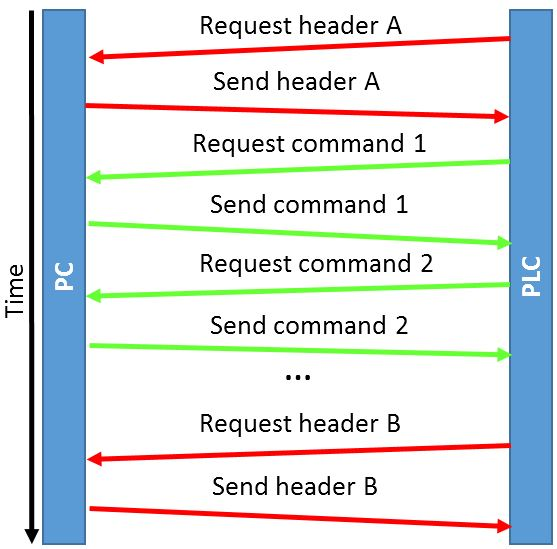
\includegraphics[width=0.4\textwidth]{figures/systemDesign/network.JPG}
	\captionof{figure}[Network interface data flow]{Data flow during communication between PC-PLC over designed network interface}
	\label{fig:network}
\end{center}

The Project Requirements stipulate that hardware control needs to be implemented on a programmable logic controller (PLC) and that the user interface needs to be on a PC. As such, some sort of networking interface needs to be implemented such that the two devices can communicate with each other. 

In the industry, PLCs are usually implemented in large scale operations with many devices and the requirements to be able to share real time data and operate on a communications standard called Open Platform Communications (OPC) (formerly known as Object Linking and Embedded (OLE) for Process Control - OPC). Unfortunately while OPC is a standard, actual OPC Server software are generally propriety and expensive, and so the decision was made to make a custom network protocol.

The link layer was chosen to be Ethernet due to physical ports being available on both PC and PLC. The transport layer was chosen to be User Datagram Protocol (UDP) due to both devices having UDP/TCP socket interfaces designed into the operating system, making them easy to use. The internet layer was chosen to be IPv4 (since maximizing the number of potential addresses wasn't needed as in IPv6).

A simple application layer protocol was designed by the DoodleBot Team. Figure ~\ref{fig:network} shows an example of basic operation of this protocol. 

The PC acts as the server and the PLC acts as a client. When in the right state, the PLC requests data from the PC. If the PC has data ready, it replies with the required data. Every packet of data includes an index of what it is to add robustness of the system (including missed packets, or asynchronous behaviour). The two directions of data flow - PC-PLC and PLC-PC operate on different ports to allow faster data transfer and to stop collisions (as could happen if reading and writing on the same port).

The first type of data packet is the header. The header tells the PLC that the PC has an image to draw and to get ready to start operating. The index is a single bit that switches between two states - this is so if operation of the PLC is stopped prematurely, it can request the same header and start the process again rather than skipping to the next image. The header then contains information on the total number of commands to expect and the sample time for the velocity profiles. The PC maintains a buffer of processed images including both headers and command lists, and only deletes old images when the PLC requests a new header.

The second type of data packet is a command. Each command contains an index of its command number within a certain image. There are then two types of commands: A 'move' command retracts the drawing head and contains an X,Y coordinate for the head to move to at a preset constant speed. Once it arrives, the next command is processed. A 'draw' command extends the drawing head and contains a velocity for X and Y to run at for the sample speed specified in the header before moving to the next command.

